% Number 830
% CAPMA Algebra Units 
% Throwing chestnuts - hard
% JG

% Watermark
\AddToShipoutPicture*{\BackgroundPic}

\addtocounter {ProbNum} {1}

%\begin{floatingfigure}[r]{.44\textwidth}
%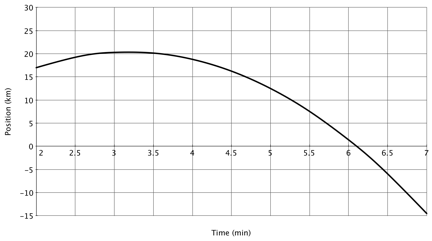
\includegraphics[scale=.5]{/Users/jgates/desktop/latex/pics/xgraph2}
%\end{floatingfigure}
 
{\bf \Large{\arabic{ProbNum}}} While sitting on a tree branch 9 meters above the ground (you're quite a climber!), you drop a chestnut.  When it's halfway to the ground, you throw a second chestnut downward.  \bigskip

What initial speed do you need to give the second chestnut so that it strikes the ground at the same time as the first chestnut?\paragraph{}
\noindent
\vfill

%\begin{center}
%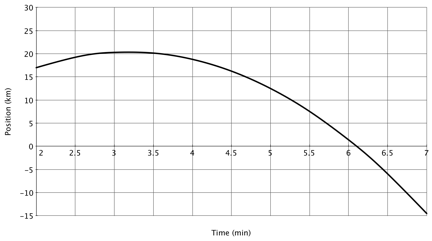
\includegraphics[scale=1]{/Users/jgates/desktop/latex/pics/xgraph2}
%\end{center}


\newpage